% Chapter 5
\section{The Other Fixed Point: Where Gradient Descent Goes When $d > n$}\label{sec:gd-underdet}

The exact solution \eqref{eq:gd-exact} of Chapter~\ref{sec:gd} has a hidden premise: $\X^\top\X$ invertible. This chapter turns to the opposite, \textbf{underdetermined} regime $d > n$: fewer equations than unknowns, so $\X^\top\X \in \R^{d \times d}$ is necessarily singular (rank $\le n < d$), the closed form \eqref{eq:ols-closed} no longer exists, and the decay matrix $\bm{I} - \eta\X^\top\X$ of Chapter~\ref{sec:gd} has $d - n$ eigenvalues identically equal to $1$ — the error \textbf{never decays} along certain directions. Yet it is precisely here that gradient descent delivers a profound result: \textbf{the iteration still converges; it converges to a special solution selected by the initialization; and starting from $\widehat{\bbeta}_0 = \zero$, it converges to the minimum-norm solution}
\[
  \widehat{\bbeta}' = \X^\top (\X \X^\top)^{-1} \y .
\]

\subsection{Setup: $d > n$, and the Solution Set Is a Manifold}\label{sec:underdet-setup}

Let $\X \in \R^{n \times d}$ have \textbf{full row rank} ($\rank(\X) = n$: the $n$ rows are linearly independent, as continuously distributed random data almost surely are). Then $\X\X^\top \in \R^{n \times n}$ is symmetric positive definite and invertible. In this case:

\begin{itemize}
  \item The system $\X \bbeta = \y$ is \textbf{consistent} ($\y$ necessarily lies in the column space), and its solutions are \textbf{not unique}: the general solution is
  \[
    \big\{ \bbeta : \X \bbeta = \y \big\} = \widehat{\bbeta}' + \mathcal{N}(\X),
    \qquad
    \mathcal{N}(\X) = \{ \bm{w} \in \R^d : \X \bm{w} = \zero \},
  \]
  a $(d - n)$-dimensional affine subspace (the solution manifold) — every point of it is an interpolating solution;
  \item The loss $L(\bbeta) = \frac{1}{2}\norm{\y - \X\bbeta}^2$ vanishes identically on this manifold: the global minimum is $0$ and is attained \textbf{on a manifold};
  \item $\X^\top\X$ has $d - n$ zero eigenvalues, and $(\X^\top\X)^{-1}$ is undefined — all the formulas of Chapter~\ref{sec:gd} fail here.
\end{itemize}

\subsection{A New Fixed Point, and Two Verifications}

\subsubsection*{Verification 1: exact interpolation}
Substitute directly:
\begin{equation}\label{eq:interp}
  \X \, \widehat{\bbeta}' = \X \X^\top (\X \X^\top)^{-1} \y = \y .
\end{equation}
That is, $\y = \X \widehat{\bbeta}'$: training error exactly zero — \textbf{interpolation}. This is the continuation, into $d > n$, of the ``zero residuals'' phenomenon at $d = n$ (Section~\ref{sec:hd-break}): excess capacity turns fitting into memorization.

\subsubsection*{Verification 2: a first-order equilibrium}
The gradient is
\begin{equation}\label{eq:grad-at-p}
  \nabla L(\widehat{\bbeta}') = \X^\top \big( \X \widehat{\bbeta}' - \y \big) = \X^\top ( \y - \y ) = \zero .
\end{equation}
So $\widehat{\bbeta}'$ is a \textbf{first-order equilibrium} (stationary point) of the least-squares loss; since $L$ is convex and $L(\widehat{\bbeta}') = 0 = \min L$, it is in fact a global minimum. Hence it is also a fixed point of the GD iteration \eqref{eq:gd}: $\widehat{\bbeta}' - \eta\, \nabla L(\widehat{\bbeta}') = \widehat{\bbeta}'$ for \textbf{every} $\eta$. Indeed \eqref{eq:grad-at-p} shows more: \textbf{every point of the entire solution manifold $\widehat{\bbeta}' + \mathcal{N}(\X)$ is a fixed point} — not an isolated equilibrium but a whole set of equilibria.

\subsection[Minimum Norm: The Point of the Solution Manifold Closest to the Origin]{Minimum Norm: $\widehat{\bbeta}'$ Is the Point of the Solution Manifold Closest to the Origin}\label{sec:minnorm}

\begin{theorem}[Minimum-norm solution]\label{thm:minnorm}
On the solution manifold $\{ \bbeta : \X \bbeta = \y \}$, $\widehat{\bbeta}' = \X^\top(\X\X^\top)^{-1}\y$ is the unique point of smallest Euclidean norm.
\end{theorem}
\begin{proof}
Take any solution $\bbeta$ and write $\bbeta = \widehat{\bbeta}' + \bm{w}$ with $\X\bm{w} = \zero$ (the difference of two solutions lies in the null space). The key observation: $\widehat{\bbeta}' \perp \mathcal{N}(\X)$, because
\[
  \langle \widehat{\bbeta}',\ \bm{w} \rangle = \y^\top (\X\X^\top)^{-1} \X\, \bm{w} = 0 .
\]
Pythagoras then gives
\[
  \norm{\bbeta}^2 = \norm{\widehat{\bbeta}'}^2 + \norm{\bm{w}}^2 \;\ge\; \norm{\widehat{\bbeta}'}^2,
\]
with equality if and only if $\bm{w} = \zero$. So $\widehat{\bbeta}'$ is exactly the point where the solution manifold meets $\mathrm{row}(\X)$ (the column space of $\X^\top$).
\end{proof}

\subsection{Stability: Contraction on the Row Space, Neutrality on the Null Space}\label{sec:stability}

The set of fixed points is large; does the iteration converge, and to what? Carry over the stability analysis of Chapter~\ref{sec:gd}, changing only the spectrum. The GD map $\bm{G}(\bbeta) = \bbeta - \eta \nabla L(\bbeta)$ — itself linear — satisfies
\[
  \bm{G}(\bbeta) - \bm{G}(\bbeta_0) = (\bm{I} - \eta \X^\top \X)(\bbeta - \bbeta_0).
\]
The eigenvalues of $\X^\top\X$: $n$ positive ones $\lambda_1 \ge \dots \ge \lambda_n > 0$ (identical to the nonzero eigenvalues of $\X\X^\top$), plus $d - n$ zeros. So the eigenvalues of $\bm{I} - \eta\X^\top\X$ are
\[
  \underbrace{1 - \eta \lambda_j}_{n \text{ of them}},\ j = 1..n;
  \qquad
  \underbrace{1}_{d - n \text{ of them}}.
\]
\begin{itemize}
  \item \textbf{Row-space directions} (the complement of the $d-n$ zero-eigenvalue directions): when $0 < \eta < \dfrac{2}{\lambda_{\max}(\X\X^\top)}$, $|1 - \eta\lambda_j| < 1$ — \textbf{contraction}, the same exponential decay as in the $n \gg d$ case;
  \item \textbf{Null-space directions}: the factor is identically $1$ — \textbf{neutral}: the $\mathcal{N}(\X)$ component of the initial error is \textbf{preserved as is, forever}.
\end{itemize}

The conclusions, stated in layers:
\begin{enumerate}[label=(\arabic*)]
  \item \textbf{Every point of the solution manifold $\widehat{\bbeta}' + \mathcal{N}(\X)$ is Lyapunov stable}: transverse (row-space) perturbations are exponentially pressed back toward the manifold, tangential (null-space) perturbations neither grow nor vanish, and the iterate stays in a bounded neighborhood of the perturbed point;
  \item As \textbf{isolated points}, none of the equilibria on the manifold is asymptotically stable (a small tangential perturbation does not return) — what is stable is \textbf{the manifold itself}: it is normally attracting;
  \item \textbf{The initialization decides the landing point}: since the null-space component is conserved, the null-space component of $\widehat{\bbeta}_0$ is carried all the way to the limit —
  \[
    \lim_{t \to \infty} \widehat{\bbeta}_t = \widehat{\bbeta}' + \underbrace{\bm{P}_{\mathcal{N}(\X)}\, \widehat{\bbeta}_0}_{\text{null-space component}} ,
  \]
  where $\bm{P}_{\mathcal{N}(\X)}$ is the orthogonal projection onto the null space.
\end{enumerate}

\subsection{The Exact Solution, Continued: GD from Zero $=$ Implicit Minimum-Norm Regularization}\label{sec:implicit}

Take the most common initialization $\widehat{\bbeta}_0 = \zero$: its null-space component is zero, and the iteration \textbf{stays in $\mathrm{row}(\X)$ for its entire run} (inductively, $\widehat{\bbeta}_t = \X^\top \bm{u}_t$ for some $\bm{u}_t$, since the gradient $\X^\top(\cdot)$ always pulls vectors back into the row space). There is only one interpolation point in the row space — $\widehat{\bbeta}'$ itself. Hence:

\begin{theorem}[Exact solution for GD in the underdetermined case]\label{thm:gd-exact-underdet}
Let $\X$ have full row rank, $0 < \eta < 2/\lambda_{\max}(\X\X^\top)$, and $\widehat{\bbeta}_0 = \zero$. Then
\begin{equation}\label{eq:gd-exact-underdet}
  \boxed{\;\widehat{\bbeta}_t = \Big[ \bm{I} - \big( \bm{I} - \eta\, \X^\top \X \big)^{t} \Big]\, \X^\top (\X \X^\top)^{-1} \y
       = \Big[ \bm{I} - \big( \bm{I} - \eta\, \X^\top \X \big)^{t} \Big]\, \widehat{\bbeta}'\;}
\end{equation}
and $\widehat{\bbeta}_t \to \widehat{\bbeta}'$ (the minimum-norm interpolating solution), with convergence rate governed by the condition number of $\X\X^\top$: $\norm{\widehat{\bbeta}_t - \widehat{\bbeta}'} = O\big( \big(\frac{\kappa - 1}{\kappa + 1}\big)^t \big)$ (at the optimal step size).
\end{theorem}
\begin{proof}
Use the identity $\X^\top (\bm{I} - \eta \X\X^\top) = (\bm{I} - \eta \X^\top\X) \X^\top$ (both sides equal $\X^\top - \eta \X^\top \X \X^\top$) to unroll \eqref{eq:gd}, obtaining $\widehat{\bbeta}_t = \X^\top \big[ \eta \sum_{k=0}^{t-1} (\bm{I} - \eta\X\X^\top)^k \big] \y$. The bracket is a geometric series of $n \times n$ matrices, and $\eta < 2/\lambda_{\max}$ keeps its spectral radius below $1$ (strict contraction of all eigenvalues), so $\eta \sum_{k<t}(\bm{I} - \eta\X\X^\top)^k = \big[ \bm{I} - (\bm{I} - \eta\X\X^\top)^t \big](\X\X^\top)^{-1}$; substituting back and reusing the identity gives \eqref{eq:gd-exact-underdet}. The limit follows from $(\bm{I} - \eta\X\X^\top)^t \to \zero$; the rate is Corollary~\ref{thm:gd-opt} verbatim, with the spectrum of $\X^\top\X$ replaced by that of $\X\X^\top$ (same nonzero eigenvalues).
\end{proof}

Place \eqref{eq:gd-exact-underdet} next to \eqref{eq:gd-exact-zero}: the structures are identical — \textbf{the only difference is the ``target'': $\bhat = (\X^\top\X)^{-1}\X^\top\y$ is replaced by $\widehat{\bbeta}' = \X^\top(\X\X^\top)^{-1}\y$}. The formal symmetry is no coincidence; the next section names the object that governs both.

\begin{remark}[Implicit regularization]
Theorem~\ref{thm:gd-exact-underdet} is the prototype of the modern theory of \emph{implicit regularization} / \emph{implicit bias}: \textbf{with no explicit penalty whatsoever, plain gradient descent from the origin automatically selects, among all interpolating solutions, the one of smallest norm — which is often the one that generalizes best}. The phenomenon that overparameterized neural networks ``memorize without exploding and still generalize'' has, in this linear version, its cleanest mathematical embodiment.
\end{remark}

\begin{figure}[htbp]
  \centering
  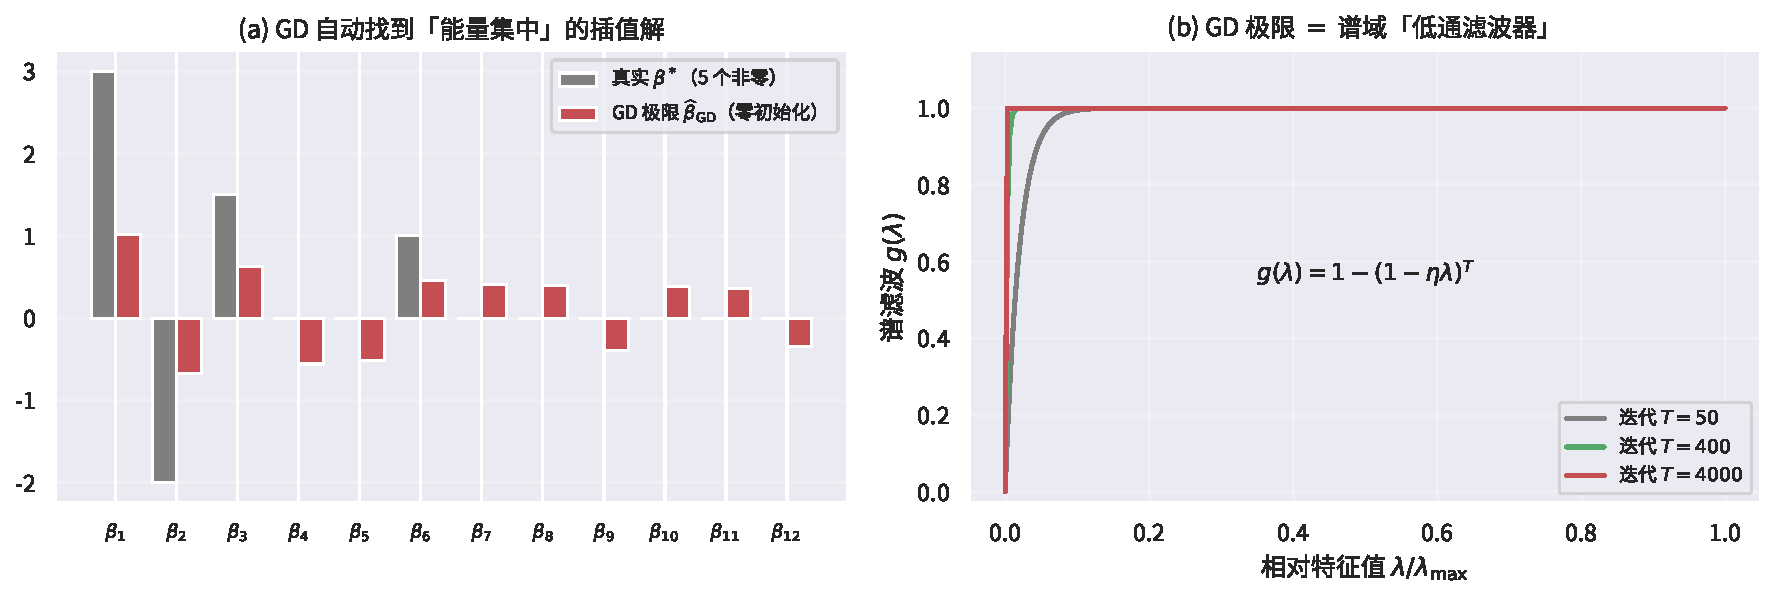
\includegraphics[width=\linewidth]{figures/ch5_implicit.pdf}
  \caption{Two faces of implicit regularization ($d = 100 > n = 30$, noiseless interpolation): (a) the limit of zero-initialized GD (red) recovers energy along the true signal directions (gray, 5 nonzero coefficients) while automatically shrinking along the noise directions; (b) the spectral-filtering interpretation — $t$ steps of GD apply the factor $g(\lambda)=1-(1-\eta\lambda)^t$ along each eigen-direction $\lambda$: large-eigenvalue directions converge first, small-eigenvalue directions last, equivalent to a ``low-pass filter.''}
  \label{fig:ch5-implicit}
\end{figure}

\subsection{Comparison with the Pseudoinverse: One Object, Several Faces}\label{sec:pseudo-compare}

Now for the comparison this chapter owes you. The Moore--Penrose pseudoinverse $\X^+$ is defined uniformly via the SVD: if $\X = \bm{U} \bm{\Sigma} \bm{V}^\top$ ($\bm{\Sigma}$ diagonal with singular values $s_j > 0$), then
\[
  \X^+ = \bm{V} \bm{\Sigma}^{+} \bm{U}^\top, \qquad
  \bm{\Sigma}^{+} \text{ replaces each } s_j \text{ by } 1/s_j \ (\text{zeros stay zero}).
\]
It yields the \textbf{minimum-norm least-squares solution} $\X^+\y$ for \textbf{any} $\X$. In the two full-rank regimes it collapses to the two familiar formulas:

\begin{itemize}
  \item \textbf{Full column rank} ($n \gg d$): $\X^+ = (\X^\top\X)^{-1}\X^\top$ — the OLS closed form of Section~\ref{sec:hd-closed};
  \item \textbf{Full row rank} ($d > n$): $\X^+ = \X^\top(\X\X^\top)^{-1}$ — \textbf{exactly this chapter's $\widehat{\bbeta}'$}. (Verify by SVD: $\X\X^\top = \bm{U}\bm{\Sigma}\bm{\Sigma}^\top\bm{U}^\top$, whose inverse is $\bm{U}(\bm{\Sigma}\bm{\Sigma}^\top)^{-1}\bm{U}^\top$; left-multiplying by $\X^\top = \bm{V}\bm{\Sigma}^\top\bm{U}^\top$ gives $\bm{V}\bm{\Sigma}^+\bm{U}^\top$.)
\end{itemize}

So: \textbf{in the full-row-rank case $d > n$, $\widehat{\bbeta}'$ \emph{is} the pseudoinverse solution} — not ``another solution,'' but the same object seen in the underdetermined regime. The table below gathers every route, appearing throughout the book, to ``the same point'':

\begin{center}
\resizebox{\linewidth}{!}{%
\begin{tabular}{@{}llll@{}}
\toprule
Object & Formula & Applies when & How it is reached \\
\midrule
OLS closed form & $(\X^\top\X)^{-1}\X^\top\y$ & $n \gg d$, full column rank & Solve the normal equations directly \\
\textbf{This chapter's $\widehat{\bbeta}'$} & $\X^\top(\X\X^\top)^{-1}\y$ & $d > n$, full row rank & Solve the interpolation equations directly \\
Pseudoinverse solution $\X^+\y$ & SVD definition & any rank & The uniform definition (parent of the two above) \\
GD, $\widehat{\bbeta}_0 = \zero$ & $\lim_t \widehat{\bbeta}_t$ & any rank & Implicit convergence to $\X^+\y$ (exact solutions of these two chapters) \\
ridge, $\lambda \to 0^+$ & $\lim_{\lambda \to 0^+}(\X^\top\X + \lambda\bm{I})^{-1}\X^\top\y$ & any rank & Equals $\X^+\y$ (limit of an identity; see exercises) \\
\bottomrule
\end{tabular}}
\end{center}

Two comparison conclusions deserve separate remembering:

\begin{enumerate}[label=(\arabic*)]
  \item \textbf{Algebraically}: $\widehat{\bbeta}' = \X^+\y$ (full row rank) — it coincides with the pseudoinverse solution \textbf{exactly}, including the ``minimum norm'' property: among all defining properties of the pseudoinverse, the condition $\X^+\y \perp \mathcal{N}(\X)$ \emph{is} Theorem~\ref{thm:minnorm} in the underdetermined case.
  \item \textbf{Dynamically}: the pseudoinverse is ``static'' (the SVD carves out the answer in one cut), GD is ``dynamic'' (a polynomial inches toward it): \eqref{eq:gd-exact-underdet} says the $t$-step GD solution equals $\big[\bm{I} - (\bm{I} - \eta\X^\top\X)^t\big]\X^+\y$, the bracket a contraction polynomial acting on the pseudoinverse solution. Change the initialization and GD lands at \textbf{other} interpolating points (carrying the initialization's null-space component) — \textit{the GD family reaches the entire solution manifold; the pseudoinverse (and the zero initialization) selects the point of the manifold closest to the origin}.
\end{enumerate}

\begin{keybox}[Chapter takeaways]
\begin{itemize}
  \item When $d > n$ with full row rank, $\widehat{\bbeta}' = \X^\top(\X\X^\top)^{-1}\y$ satisfies (i) exact interpolation $\X\widehat{\bbeta}' = \y$ and (ii) $\nabla L(\widehat{\bbeta}') = \zero$ (first-order equilibrium), and is the \textbf{unique minimum-norm} point of the solution manifold;
  \item The entire solution manifold $\widehat{\bbeta}' + \mathcal{N}(\X)$ consists of GD fixed points: row-space directions contract exponentially (for $0 < \eta < 2/\lambda_{\max}(\X\X^\top)$), null-space directions are neutral — the manifold is transversally attracting, its points only Lyapunov stable, and the landing point is decided by the initialization's null-space component;
  \item Exact solution $\widehat{\bbeta}_t = [\bm{I} - (\bm{I} - \eta\X^\top\X)^t]\widehat{\bbeta}'$: structurally isomorphic to the $n \gg d$ case, with the target switched from $\bhat$ to $\widehat{\bbeta}'$; for $\widehat{\bbeta}_0 = \zero$, GD converges \textbf{implicitly} to the minimum-norm solution — the linear prototype of implicit regularization;
  \item Relation to the pseudoinverse: with full row rank, $\widehat{\bbeta}' = \X^+\y$ identically; the pseudoinverse, the two closed forms, the GD-from-zero limit, and the ridge zero limit are \textbf{five faces of one minimum-norm least-squares solution}.
\end{itemize}
\end{keybox}

\begin{exercise}\label{ex:ridge-dual}
Prove the identity $(\X^\top\X + \lambda\bm{I})^{-1}\X^\top = \X^\top(\X\X^\top + \lambda\bm{I})^{-1}$ (multiply both sides by $(\X^\top\X + \lambda\bm{I})$ and rearrange), and use it to show that the ridge solution converges to $\X^+\y$ as $\lambda \to 0^+$ (no full-rank assumption needed).
\end{exercise}

\begin{exercise}\label{ex:gd-limit-anyinit}
Let $d > n$ with $\X$ of full row rank. Show that for any initialization $\widehat{\bbeta}_0$, the GD limit is $\widehat{\bbeta}' + \bm{P}_{\mathcal{N}(\X)} \widehat{\bbeta}_0$, where $\bm{P}_{\mathcal{N}(\X)} = \bm{I} - \X^+\X$ is the orthogonal projection onto the null space; and explain why this is consistent with Theorem~\ref{thm:gd-exact-underdet}.
\end{exercise}

\begin{exercise}\label{ex:spectrum}
Compare the ``effective dimension'' of the two regimes: for $n \gg d$, the GD error decay is governed by the $d$ eigenvalues of $\X^\top\X$; for $d > n$, by the $n$ eigenvalues of $\X\X^\top$. Prove that the two matrices have exactly the same nonzero eigenvalues (hint: if $\X^\top\X \bm{v} = \lambda \bm{v}$, look at $\X \bm{v}$), and explain why this spectral identity lets the convergence-rate formulas of the two chapters be interchanged.
\end{exercise}
